\documentclass[aspectratio=169,10pt]{beamer}
\usetheme{metropolis}
\usepackage{booktabs}
\usepackage{graphicx}
\usepackage{amsmath}
\usepackage{xcolor}
\usepackage{tikz}
\usetikzlibrary{arrows.meta,positioning}

\definecolor{good}{RGB}{39,174,96}
\definecolor{warn}{RGB}{192,57,43}
\definecolor{muted}{RGB}{120,120,120}
\definecolor{accent}{RGB}{46,106,178}

\setbeamertemplate{footline}{%
  \hfill\insertframenumber/\inserttotalframenumber\hspace*{1em}\vspace*{0.5em}}

% ─────────────────────────────────────────────────────────────────────────────
\title{EB-JEPA for EEG Time Series}
\subtitle{Self-Supervised Abnormality Detection on TUAB}
\author{tcourtois \and yhammache \and tvasnier}
\date{Hackathon — June 2026}
% ─────────────────────────────────────────────────────────────────────────────

\begin{document}
\maketitle

% ─────────────────────────────────────────────────────────────────────────────
\begin{frame}{Task \& Motivation}
\begin{columns}[T]
\column{0.55\textwidth}
\textbf{TUAB} — TUH Abnormal EEG Corpus
\begin{itemize}
  \item Binary: normal / abnormal clinical EEG
  \item 19 channels, 200\,Hz, 10\,s windows
  \item 2717 train / 276 eval recordings
  \item Patient-disjoint split — no leakage
\end{itemize}

\vspace{0.6em}
\textbf{Challenge:} learn a transferable EEG representation \emph{without} labels
\begin{itemize}
  \item Labelling EEG requires licensed neurologists
  \item Unlabelled data is abundant
  \item Can self-supervised learning close the gap?
\end{itemize}

\column{0.42\textwidth}
\begin{center}
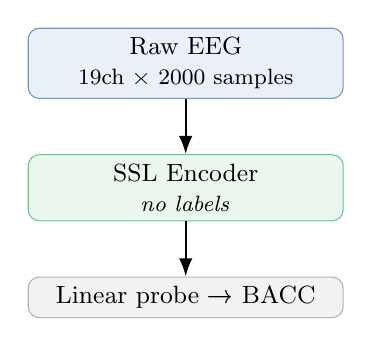
\begin{tikzpicture}[font=\small, node distance=0.7cm]
  \node[draw=accent!70, fill=accent!10, rounded corners, minimum width=4cm, align=center]
    (raw) {Raw EEG\\ \footnotesize 19ch × 2000 samples};
  \node[draw=good!70, fill=good!10, rounded corners, below=of raw, minimum width=4cm, align=center]
    (enc) {SSL Encoder\\ \footnotesize \emph{no labels}};
  \node[draw=gray!60, fill=gray!10, rounded corners, below=of enc, minimum width=4cm, align=center]
    (probe) {Linear probe → BACC};
  \draw[-{Latex}, thick] (raw) -- (enc);
  \draw[-{Latex}, thick] (enc) -- (probe);
\end{tikzpicture}
\end{center}
\end{columns}
\end{frame}

% ─────────────────────────────────────────────────────────────────────────────
\begin{frame}{Our Approach — EB-JEPA Two-View SSL}

\begin{columns}[T]
\column{0.55\textwidth}
\textbf{Energy-Based JEPA} (two-view invariance):
\begin{itemize}
  \item Take one EEG window; create two \emph{augmented views}
  \item Push both through the same encoder $f_\theta$
  \item Force $z_1 \approx z_2$ while preventing collapse
\end{itemize}

\vspace{0.5em}
\textbf{Augmentations:}
\begin{itemize}
  \item Gaussian noise, amplitude jitter, channel drop
  \item \textbf{+ Corruption} (our design): 20\% time masking, $\pm6\sigma$ spike injection
\end{itemize}

\vspace{0.5em}
\textbf{What we contributed:}
\begin{itemize}
  \item 4 encoder architectures
  \item 2 SSL objectives (VICReg / SIGReg)
  \item Full ablation + bug diagnosis
  \item Honest evaluation protocol
\end{itemize}

\column{0.42\textwidth}
\begin{center}
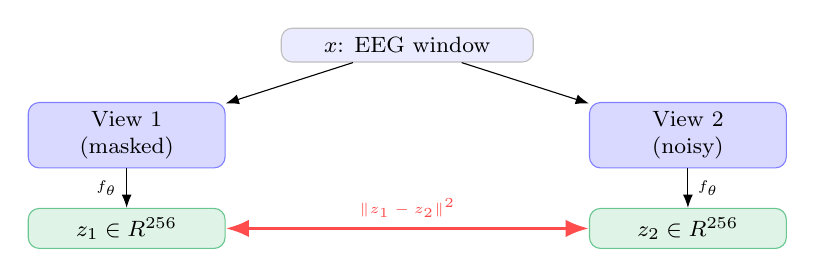
\begin{tikzpicture}[font=\footnotesize, node distance=0.5cm and 0.7cm]
  \node[draw=gray!50, fill=blue!8, rounded corners, minimum width=3.2cm, align=center]
    (x) {$x$: EEG window};
  \node[draw=blue!50, fill=blue!15, rounded corners, below left=of x, minimum width=2.5cm, align=center]
    (v1) {View 1\\ (masked)};
  \node[draw=blue!50, fill=blue!15, rounded corners, below right=of x, minimum width=2.5cm, align=center]
    (v2) {View 2\\ (noisy)};
  \node[draw=good!70, fill=good!15, rounded corners, below=0.5cm of v1, minimum width=2.5cm, align=center]
    (z1) {$z_1 \in \mathbb{R}^{256}$};
  \node[draw=good!70, fill=good!15, rounded corners, below=0.5cm of v2, minimum width=2.5cm, align=center]
    (z2) {$z_2 \in \mathbb{R}^{256}$};
  \draw[-{Latex}] (x) -- (v1); \draw[-{Latex}] (x) -- (v2);
  \draw[-{Latex}] (v1) -- (z1) node[midway,left,font=\tiny]{$f_\theta$};
  \draw[-{Latex}] (v2) -- (z2) node[midway,right,font=\tiny]{$f_\theta$};
  \draw[{Latex}-{Latex}, red!70, very thick] (z1.east) -- (z2.west)
    node[midway, above, font=\tiny\bfseries, text=red!70]{$\|z_1-z_2\|^2$};
\end{tikzpicture}
\end{center}
\end{columns}
\end{frame}

% ─────────────────────────────────────────────────────────────────────────────
\begin{frame}{Four Encoder Architectures}

\begin{tabular}{llll}
\toprule
\textbf{Encoder} & \textbf{Tokenisation} & \textbf{Architecture} & \textbf{Params} \\
\midrule
\textbf{Conv} & Strided Conv1D ($k$=7) & 4 BN+GELU blocks & 0.4M \\
\textbf{LaBraM} & 1s patches per channel & ViT (190 tokens) & 1.2M \\
\textbf{BIOT} & FFT magnitude patches & ViT (190 tokens) & 1.2M \\
\textbf{EEGPT} & Cross-ch pool → 10 tokens & Temporal transformer & 0.8M \\
\bottomrule
\end{tabular}

\vspace{0.8em}
\begin{columns}[T]
\column{0.48\textwidth}
\textbf{VICReg} loss (Bardes et al. 2022):
$$\mathcal{L} = 25\underbrace{\|z_1-z_2\|^2}_{\text{invariance}} + 25\,V + 1\,C$$
Hinge variance + off-diagonal covariance penalty.

\column{0.48\textwidth}
\textbf{SIGReg / BCS}:
Replaces $V$+$C$ with Epps–Pulley Gaussianity test on random projections.
Stronger anti-collapse, less hyperparameter-sensitive.
\end{columns}
\end{frame}

% ─────────────────────────────────────────────────────────────────────────────
\begin{frame}[fragile]{The Evaluation Trap}

\begin{alertblock}{Per-window vs Per-recording — 5 pp difference, same encoder}
\begin{itemize}
  \item \textbf{Literature} (BIOT, LaBraM, FEMBA, EEGPT): reports \textbf{per-window} — each 10\,s segment is a separate test point. Up to 409\,455 test samples from 2339 recordings.
  \item \textbf{Our evaluation}: mean-pools 16 windows per patient into one embedding → \textbf{per-recording} score.
  \item Per-recording is $\approx$5\,pp \emph{higher} than per-window for the same encoder (noise averaging).
\end{itemize}
\end{alertblock}

\vspace{0.4em}
\begin{block}{Our initial mistake}
We reported per-recording BACC \textbf{0.836} against LaBraM's per-window BACC \textbf{0.814}
and concluded ``we match LaBraM.'' That comparison is invalid.\\[4pt]
\textbf{Correction}: our best \emph{per-window} score is \textbf{0.775} — below BIOT (0.802) and LaBraM (0.814).
\end{block}

\vspace{0.4em}
\textcolor{muted}{\footnotesize Note: per-recording is arguably the right \emph{clinical} metric (you classify patients, not 10s snippets), but it is not what the benchmark measures.}
\end{frame}

% ─────────────────────────────────────────────────────────────────────────────
\begin{frame}{Results — Fair Per-Window Comparison}

\begin{columns}[T]
\column{0.52\textwidth}
\begin{tabular}{lcc}
\toprule
Method & BACC & AUROC \\
\midrule
\textcolor{muted}{ContraWR} & \textcolor{muted}{0.775} & \textcolor{muted}{0.846} \\
\textcolor{accent}{BIOT pretrained} & \textcolor{accent}{0.802} & \textcolor{accent}{0.874} \\
\textcolor{accent}{LaBraM-Base} & \textcolor{accent}{0.814} & \textcolor{accent}{0.902} \\
\midrule
EB-JEPA base & 0.756 & 0.845 \\
\textbf{+ corruption} & \textbf{0.770} & 0.848 \\
\textbf{+ SIGReg + corrupt} & \textbf{0.775} & \textbf{0.856} \\
EEGNet (supervised) & 0.796 & 0.882 \\
\bottomrule
\end{tabular}

\vspace{0.5em}
\textcolor{good}{$\checkmark$} Matches ContraWR — competitive SSL baseline\\
\textcolor{warn}{$\times$} Still 4\,pp below LaBraM

\column{0.45\textwidth}
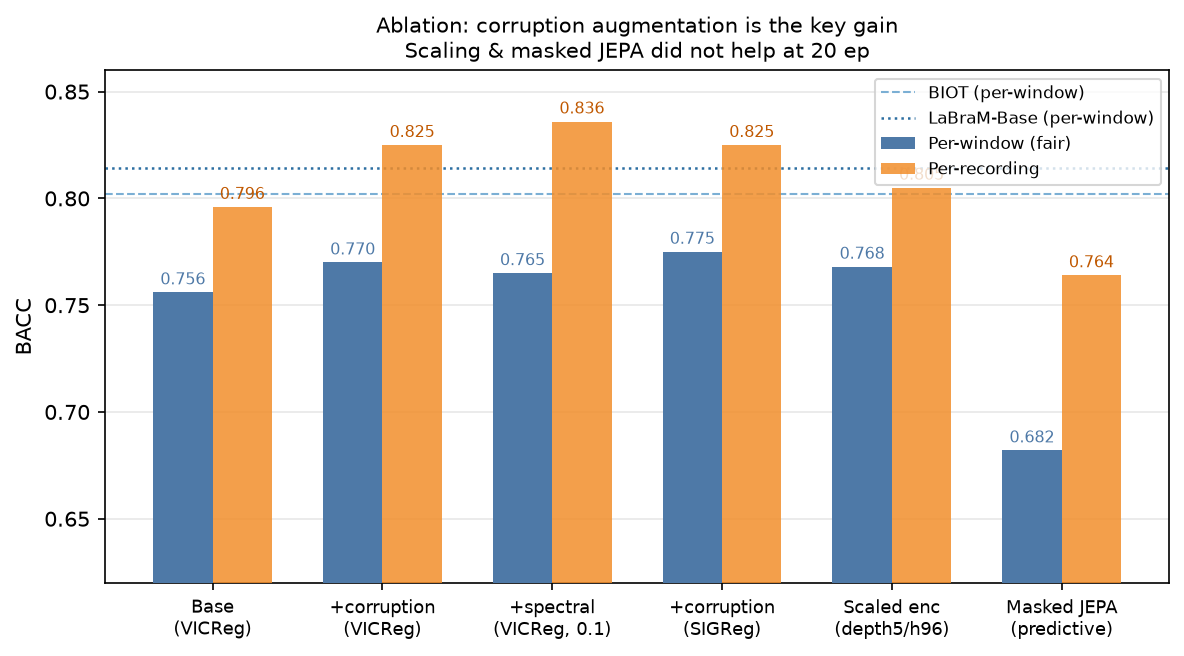
\includegraphics[width=\linewidth]{figures/ablation_what_moved.png}
\end{columns}
\end{frame}

% ─────────────────────────────────────────────────────────────────────────────
\begin{frame}{Ablation — What Actually Moved the Needle}

\begin{columns}[T]
\column{0.6\textwidth}
\begin{tabular}{lcc}
\toprule
Variant & $\Delta$BACC & $\Delta$AUROC \\
\midrule
Base VICReg & — & — \\
\textbf{+corruption} & \textcolor{good}{+0.014} & \textcolor{good}{+0.003} \\
+spectral (0.1) & +0.009 & +0.004 \\
SIGReg +corrupt & +0.019 & +0.011 \\
\midrule
Scaled encoder (depth 5) & $\approx$0 & — \\
150-epoch pretraining & $\approx$0 & — \\
Masked-prediction JEPA & \textcolor{warn}{$-$0.074} & — \\
Multi-corpus 4× data & +0.012 & — \\
\bottomrule
\end{tabular}

\column{0.38\textwidth}
\textbf{Key lesson:}
\begin{itemize}
  \item Corruption augmentation is the dominant win
  \item SIGReg $\geq$ VICReg (consistent with paper)
  \item Scaling \& more data did \emph{not} help — binding constraint is \textbf{encoder capacity}
  \item Frame-prediction JEPA underperformed with global-pool probe
\end{itemize}
\end{columns}
\end{frame}

% ─────────────────────────────────────────────────────────────────────────────
\begin{frame}{Failure Analysis — VICReg Bug + EEGPT Collapse}

\begin{columns}[T]
\column{0.50\textwidth}
\textbf{Bug: wrong VICReg coefficients}
\begin{itemize}
  \item Implementation used $(1,1,1)$ instead of $(25,25,1)$
  \item Invariance underweighted \textbf{25$\times$} — encoder barely penalised for mismatching views
  \item Fix: added \texttt{inv\_coeff=25} to \texttt{VICRegLoss}
\end{itemize}

\vspace{0.5em}
\textbf{EEGPT collapse (two causes)}
\begin{enumerate}
  \item \textbf{Architectural}: 19 channels → 1 pooled token per patch. Only 10 temporal tokens total. Channel-drop augmentation makes the two views structurally incompatible \emph{before} the transformer sees them.
  \item \textbf{Underweighted invariance} (the bug above): optimizer never forced the encoder to fix this.
\end{enumerate}
Result: EEGPT trained \emph{below} random init (acc 0.641 vs random 0.674).

\column{0.48\textwidth}
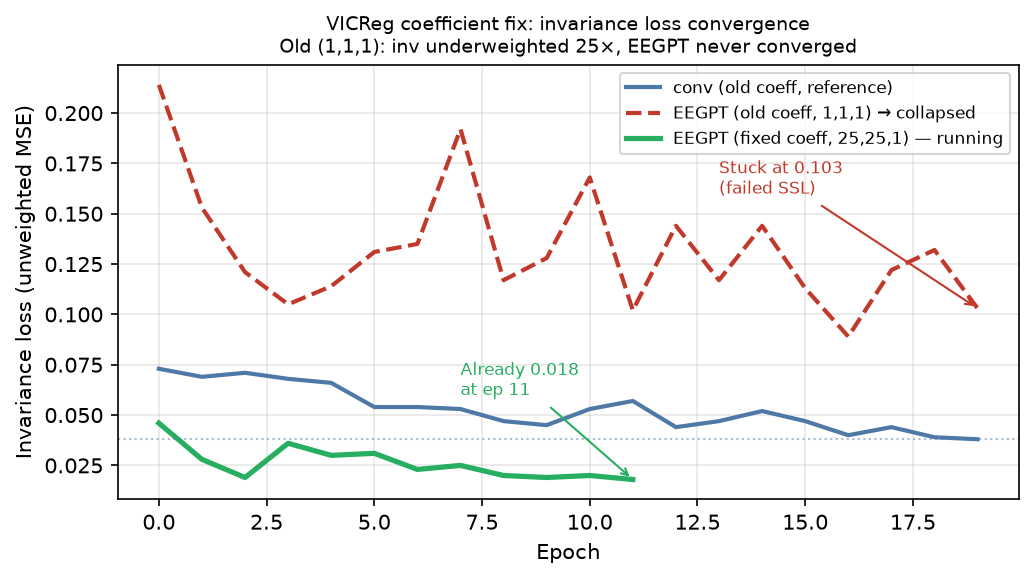
\includegraphics[width=\linewidth]{figures/vicreg_fix.png}
\footnotesize
Fixed run (green): inv\_loss 0.018 at epoch 11\\
Old run (red dashed): stuck at 0.103 at epoch 19
\end{columns}
\end{frame}

% ─────────────────────────────────────────────────────────────────────────────
\begin{frame}{Encoder Ranking \& Collapse Diagnosis}

\begin{columns}[T]
\column{0.55\textwidth}

\includegraphics[width=\linewidth]{figures/encoder_comparison.png}

\column{0.42\textwidth}
\textbf{Observations:}
\begin{itemize}
  \item \textcolor{good}{\textbf{Conv}} (simple, 0.4M) beats all transformers
  \item \textcolor{accent}{LaBraM-style} (raw patches) is the best transformer architecture for VICReg
  \item \textcolor{warn}{BIOT}: FFT magnitude discards phase → representation captures frequency statistics, not temporal pathology patterns. Slightly below random with SIGReg.
  \item \textcolor{warn}{EEGPT}: systematic collapse with old VICReg coefficients. Fix running — inv\_loss already $5\times$ lower.
\end{itemize}
\textcolor{muted}{\footnotesize Note: accuracy only for this plot (BACC unavailable for yhammache's old runs).}
\end{columns}
\end{frame}

% ─────────────────────────────────────────────────────────────────────────────
\begin{frame}{Transfer to TUEV (6-class Event Classification)}

\begin{columns}[T]
\column{0.55\textwidth}
\textbf{Task}: TUEV — 6 EEG event types (spsw, gped, pled, eyem, artf, bckg)\\
\textbf{Protocol}: freeze TUAB-pretrained encoder; train linear probe on TUEV

\vspace{0.5em}
\begin{tabular}{lcc}
\toprule
Encoder & BACC & Kappa \\
\midrule
Random init & 0.337 & 0.110 \\
\textbf{EB-JEPA (TUAB frozen)} & \textbf{0.364} & \textbf{0.141} \\
\midrule
BIOT (paper) & 0.528 & 0.435 \\
\bottomrule
\end{tabular}

\column{0.42\textwidth}
\textbf{Takeaways:}
\begin{itemize}
  \item SSL representation \emph{does} transfer — $+$0.027 BACC over random
  \item Still far below BIOT (0.528)
  \item BIOT's FFT tokenisation may be better for TUEV's frequency-based event types
  \item Pretraining task (binary pathology) $\neq$ transfer task (6 event types)
\end{itemize}
\end{columns}
\end{frame}

% ─────────────────────────────────────────────────────────────────────────────
\begin{frame}{Conclusion}

\begin{columns}[T]
\column{0.50\textwidth}
\textbf{\textcolor{good}{What works}}
\begin{itemize}
  \item Corruption augmentation: $+$0.014 BACC (dominant gain)
  \item SIGReg $\geq$ VICReg with correct $(25,25,1)$ coefficients
  \item Simple Conv encoder beats all transformer variants (3× smaller)
  \item Frozen probe BACC 0.775 matches ContraWR
  \item Per-recording BACC 0.836 — competitive clinical score
\end{itemize}

\column{0.48\textwidth}
\textbf{\textcolor{warn}{What doesn't}}
\begin{itemize}
  \item Scaling encoder: bottleneck is architecture, not width/depth
  \item EEGPT: channel-pool + channel-drop = incompatible
  \item Masked-prediction JEPA (20 ep, global-pool probe)
  \item FFT tokenisation (BIOT): discards phase/temporal dynamics
\end{itemize}
\end{columns}

\vspace{0.6em}
\begin{block}{Honest position (per-window, fair to literature)}
0.775 — below BIOT (0.802) and LaBraM (0.814). \\
Competitive with supervised EEGNet (0.796) as a \emph{frozen} representation. \\
The binding constraint is encoder capacity and tokenisation quality.
\end{block}
\end{frame}

% ─────────────────────────────────────────────────────────────────────────────
%% ─ BACKUP SLIDES ─────────────────────────────────────────────────────────────
%\begin{frame}{Backup — Per-Recording Table (Clinical)}
%\begin{tabular}{lccc}
%\toprule
%Model & BACC & AUROC & F1 \\
%\midrule
%EB-JEPA base (frozen) & 0.796 & 0.888 & 0.774 \\
%EB-JEPA +corruption & 0.825 & 0.904 & 0.805 \\
%EB-JEPA +spectral 0.1 & 0.836 & 0.887 & 0.818 \\
%EB-JEPA fine-tune & 0.837 & 0.919 & 0.816 \\
%EEGNet (supervised) & 0.824 & 0.913 & 0.802 \\
%ShallowConvNet (supervised) & 0.803 & 0.893 & 0.786 \\
%\bottomrule
%\end{tabular}
%
%\vspace{0.5em}
%\footnotesize Per-recording = mean-pool 16 windows/patient. Not comparable to per-window literature. \\
%Shown for clinical context only.
%\end{frame}

%\begin{frame}{Backup — SOTA Table (per-window, verified from PDFs)}
%\begin{tabular}{lcc}
%\toprule
%Method & BACC & AUROC \\
%\midrule
%SPaRCNet & 0.790 & 0.855 \\
%ContraWR & 0.775 & 0.846 \\
%CNN-Transformer & 0.787 & 0.850 \\
%FFCL & 0.776 & 0.844 \\
%ST-Transformer & 0.797 & 0.871 \\
%AFTA & 0.788 & 0.868 \\
%FEMBA & 0.808 & 0.882 \\
%BIOT & 0.802 & 0.874 \\
%LaBraM-Base & 0.814 & 0.902 \\
%LaBraM-Huge & 0.826 & 0.916 \\
%\bottomrule
%\end{tabular}
%\end{frame}

\end{document}
